\documentclass{article}

\usepackage[margin=1in]{geometry}
\usepackage[utf8]{inputenc}
\usepackage[english]{babel}
\usepackage[normalem]{ulem}
\usepackage{amsthm} %lets us use \begin{proof}
\usepackage{amssymb} %gives us the character \varnothing
\usepackage{xcolor}
\usepackage{float}
\usepackage{braket}
\usepackage{multirow}
\usepackage{array}
\usepackage{mathtools}
\usepackage{graphicx}

\title{Chem231B: Fake Final} % Title of the assignment

\begin{document}

\maketitle

\section*{Applications of Quantum Mechanics}

You need only do 20 questions, i.e., you can drop 2. Answer the explanation questions in complete
sentences, and comment on nontrivial steps in any of your calculations. You might want to know:
1 Hartree is 27.2114 eV, or 627.5 kcal/mol or 2625.2 kJ/mol. 1 eV is also 8065 cm$^{-1}$ or 11,604K.
The Morse potential is
\begin{equation}
  V(R) = A(\text{exp}(-2\alpha(R-R_e))-2\text{exp}(-\alpha(R-R_e)),
\end{equation}
with known eigenenergies:
\begin{equation}
  \epsilon_n = -A(1 - \frac{\alpha(n+1/2)}{\sqrt{2m\,A}})^2
\end{equation}

\noindent a) Give the Hamiltonian for an electron in a He$^+$ ion in atomic units.

{\color{blue}
  \begin{equation*}
    \hat{H} = -\frac{\nabla^2}{2} - \frac{2}{|\vec{r}|}
  \end{equation*}

  The He$^+$ is placed at the orgin. $\nabla^2$ is the Laplacian in spherical coordinates and
  $\vec{r}$ is the position of the electron.
}
\\

\noindent b) Give the kinetic and potential energies when the electron is in its ground state
in the previous problem.
\\

{\color{blue} $\langle \hat{T} \rangle = 2$ Hartree and $\langle \hat{V} \rangle = -4$ Hartree.}
\\

\noindent c) Give the Hamiltonian for the electrons in H$_2$.

{\color{blue}
  \begin{align*}
    \hat{H} & = \sum_{i=1}^2\hat{h}(i) + \hat{V}_{\text{ee}} \\
    \hat{h}(i) & = -\frac{\nabla_i^2}{2} - \frac{1}{|\vec{r}_i|} -\frac{1}{|\vec{r}_i - R\hat{z}|} \\
    \hat{V}_{\text{ee}} & = \frac{1}{2}\sum_{i\neq j} \frac{1}{|\vec{r}_i-\vec{r}_j|}
  \end{align*}

  Diatomic H$_2$ molecule is placed along the $z$-axis. $\hat{h}(i)$ is the one-electron
  operator and the $\hat{V}_{\text{ee}}$ is the two-electron operator. $r_i$ is the position
  of the electron and $R$ is the separation of the hydrogen atoms.
}
\\

\noindent d) An electron is in a 2p state. What are the possible values of $s$, $m_s$, $l$,
$m_l$, $j$, and $m_j$, where $\mathbf{j} = \mathbf{l} + \mathbf{s}$?
\\

{\color{blue} $s=1/2$, $m_s=\pm 1/2$, $l=1$, $m_l=\{-1,0,1\}$, $j=\{1/2,3/2\}$, and
  $m_j = \{\pm3/2,\pm1/2\},\{\pm1/2\}$.
}
\\

\noindent e) Find $[[l_x,l_y],l_z]$.
\\

{\color{blue}
  $[l_x,l_y] = i\hbar l_z$ and therefore, $[[l_x,l_y],l_z] = 0$
}
\\

\noindent f) How many nodes are in a 4d orbital? State which are radial, and which are
angular.
\\

{\color{blue} There are 3 total nodes in a 4d orbital. 2 are angular nodes and 1 is a
  radial node.
}
\\

\noindent g) What is the degeneracy of the level with energy $-1/18$ Hartree in a H
atom? Include spin.
\\

{\color{blue} $n=3$ and hence, there are 3s, 3p, and 3d orbitals. Considering spin,
  the degeneracy with energy $-1/18$ Hartree in a H atom is
  18.}
\\

\noindent h) What is the expectation value of $\langle 1/r \rangle$, as a function of
$\zeta$, of the trial wavefunction exp$(-\zeta r)$? (Make sure you normalize.)
\\

{\color{blue} Normalized wavefunction $\frac{\zeta^{3/2}}{\sqrt{\pi}}e^{-\zeta r}$
  and $\langle 1/r \rangle = \zeta$.
}
\\

\noindent i) Give the value of $\langle 3,2|\hat{j}_x|3,1\rangle$.

{\color{blue} 
  \begin{align*}
    \hat{j}_x & = 1/2(j_+ + j_-) \\
    \langle 3,2|\hat{j}_x|3,1\rangle & = 1/2\langle 3,2|(j_++j_-)|3,1\rangle \\
    & = 1/2\langle 3,2|\hat{j}_+|3,1\rangle \\
    & = \frac{\sqrt{10}}{2}
  \end{align*}
}
\\

\noindent j) Give the possible states $j_1 = 1/2$, $j_2 = 1$, labeled by their total
angular momentum and its $z$-component.
\\

{\color{blue} $\vec{j}=\vec{j}_1+\vec{j}_2$; $j=\{3/2,1/2\}$;
  $|3/2,\pm 3/2\rangle, |3/2,\pm 1/2\rangle, |1/2,\pm 1/2\rangle$
}
\\

\noindent k) Give the terms of the lowest configuration of C, and state which should
be the ground-state.
\\

{\color{blue} $^3P <\, ^1D <\, ^1S$}
\\

\noindent l) In the previous question, state which levels appear due to spin orbit
coupling.
\\

{\color{blue} $^3P$; $S=1$; $J=\{2,1,0\}$, spin orbit coupling splits into 3 levels}
\\

\noindent m) Write an expression for the lowest HF wavefunction of He, including both
spatial and spin parts. How does it change when coordinates 1 and 2 are swapped?

{\color{blue}
  \begin{equation*}
    \Psi^{\text{HF}}(r_1,r_2) = \frac{1}{\sqrt{2}}\phi(r_1)
    \phi(r_2)(|\upharpoonleft\downharpoonright\rangle -
    |\downharpoonleft\upharpoonright\rangle)
  \end{equation*}
  
  The spatial orbitals $\phi_1(x)$ and $\phi_2(x)$ with
  electrons $r_1$ and $r_2$. $\Psi^{\text{HF}}(r_1,r_2) = -\Psi^{\text{HF}}(r_2,r_1)$
}\\

\noindent n) Esimate the electronic repulsive energy in Be$^{++}$.

{\color{blue}
  \begin{align*}
    U_H & = \frac{5\gamma}{4} \\
    V_{ee} & = \frac{U_H}{2} = \frac{5\gamma}{8} \\
    \gamma & = Z - \frac{5}{16} = 4 - \frac{5}{16} = \frac{59}{16} \\
    V_{ee} & \approx \frac{295}{128} = 2.305\text{ Hartree}
  \end{align*}
}   

\noindent o) Why do HF calculations typically underestimate binding energies?
\\

{\color{blue} It is missing correlation energy, which is negative and
  of greater magnitude with more electron pairs.
}
\\

\noindent p) State the variational principle.
\\

{\color{blue} $E_0 \leq \langle\psi|\hat{H}|\psi\rangle = E$ where $E_0$ is the exact
  ground-state energy and $\psi$ is any nomalized ``trial wavefunction'' that can be adjusted with
  parameters minimizing the energy $E$.
}\\

\noindent q) Use the variational principle to define the universal part of the density
functional in DFT for the ground-state of electronic systems.

{\color{blue}
  \begin{align*}
    F[n] = \min_{\Psi\rightarrow n}\langle \Psi|\hat{T} + \hat{V}_{ee}|\Psi\rangle,
  \end{align*}
  $\Psi$ is antisymmetric and normalized
}\\

\noindent r) Sketch the shapes of the overlap of two atomic 2p-orbitals perpendicular
to the bond direction. State how many nodes, what shape the nodes are, and give the
symmetry labels of these orbitals.
\\

\begin{figure}[H]
  \centering
  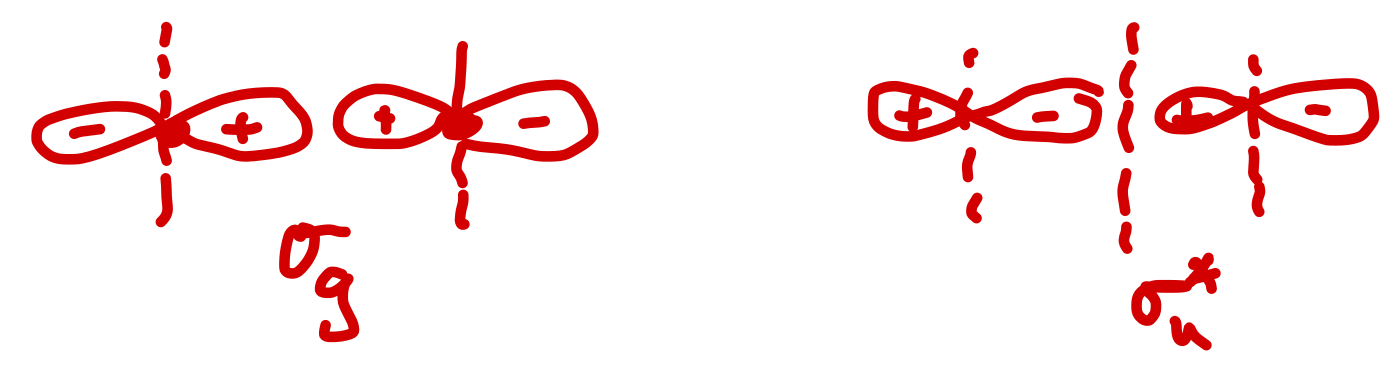
\includegraphics[scale=0.15]{p.png}
\end{figure}

\noindent s) Write the equation that determines the density for any number of same-spin
particles in a one-dimensional potential when the local density approximation is used
for the kinetic energy, and say how any constants are chosen.
\\

{\color{blue}
  \begin{center}
  n(x) =
  \begin{cases}
    1/\pi\sqrt{2(\mu - V(x))},&  \mu\geq V(x)\\
    0,              & \text{otherwise}
  \end{cases}
  \end{center}

  \begin{align*}
    \int^{\infty}_{-\infty} dx \, n(x) = N
  \end{align*}
  which determins $\mu$.
}
\\

\noindent t) The vibrational frequency of LiH is 1406 cm$^{-1}$, and its dissociation
energy is 2.43 eV. What will the dissociation energy be for LiD?
\\

{\color{blue}
  \begin{align*}
    \mu_{\text{LiH}} & = 7/8 \\
    \mu_{\text{LiD}} & = 14/9 \\
    \omega & = \sqrt{\frac{k}{\mu}} \\
    \omega_{\text{LiH}}/\omega_{\text{LiD}} & = 4/3 \\
    \omega_{\text{LiD}} & = 1054.5 \text{ cm}^{-1}
  \end{align*}

  Dissociation energy is Approximately 0.043 eV higher for LiD.
}

\noindent u) For He$_2^+$, what is the bond order and lowest energy term?
\\

{\color{blue} Bond order of 0.5 and $^2\Sigma_g$.}
\\

\noindent v) For H$_2^+$, sketch the overlap of the atomic orbitals in a minimal basis
calculation as a function of R, giving the value at $R=0$.
\\

{\color{blue} At $R=0$, the overlap of the atomic orbital is 1.}
\begin{figure}[H]
  \centering
  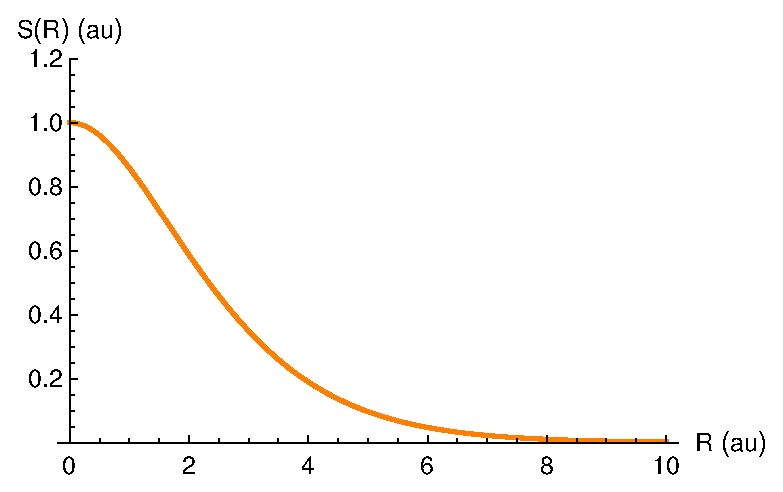
\includegraphics[scale=0.75]{h2.eps}
  \label{fig:overlap}
\end{figure}

\noindent w) For a particle in a cubic potential ($v(x) = C|x|^3$), what is the ratio
of potential to kinetic energy?
\\

{\color{blue} $\langle V\rangle/\langle T \rangle = 2/3$}
\\

\noindent x) The binding energy curve of a diatomic is often crudely approximated by a
Lennard-Jones potential:
\begin{equation*}
  U(R) = U(\infty) +D\Bigg(\Bigg(\frac{R_e}{R}\Bigg)^{12} - 2\Bigg(\frac{R_e}{R}\Bigg)^6\Bigg).
\end{equation*}

Derive an expression for the electronic potential energy as a function of $R$.

{\color{blue}
  \begin{align*}
    \langle V \rangle & = 2U + R\frac{dU}{dR} \\
    & = 2U(\infty) - 10D\Bigg(\frac{R_e}{R}\Bigg)^{12} + 8D\Bigg(\frac{R_e}{R}\Bigg)^6 \\
    & = V_{el} + V_{NN} \\
    V_{el} & = 2(\infty) -\frac{Z_AZ_B}{R} -2D\Bigg(5\Bigg(\frac{R_e}{R}\Bigg)^{12}-4\Bigg(\frac{R_e}{R}\Bigg)^6\Bigg)
  \end{align*}
}


\end{document}
